\documentclass{article}
\usepackage[T1]{fontenc}
\usepackage{lmodern}
\usepackage{graphicx}
\usepackage{amsmath,amssymb}
\usepackage[a4paper,margin=2cm]{geometry}
\usepackage[absolute,overlay]{textpos}
\setlength{\TPHorizModule}{1mm}
\setlength{\TPVertModule}{1mm}
\usepackage[indonesian]{babel}
\usepackage{hyperref}
\setlength{\emergencystretch}{2em}
% unit: Halaman 59

\begin{document}

% === Halaman 59 (llm) ===

\vspace{50mm}

Jadi, \( x^{13} + x^{11} + x^9 + x^8 + x^6 + x^5 + x^4 + x^3 + 1 \pmod{f(x)} = x^7 + x^6 + 1 = 11000001 \)

% deskripsi: Proses pembagian polinomial dalam aritmatika biner (GF(2)) untuk mencari sisa pembagian (modulo).
% bbox normalisasi: [0.0600, 0.1080, 0.9400, 0.9120]
\begin{textblock*}{184.80mm}(12.60mm,32.08mm)
\noindent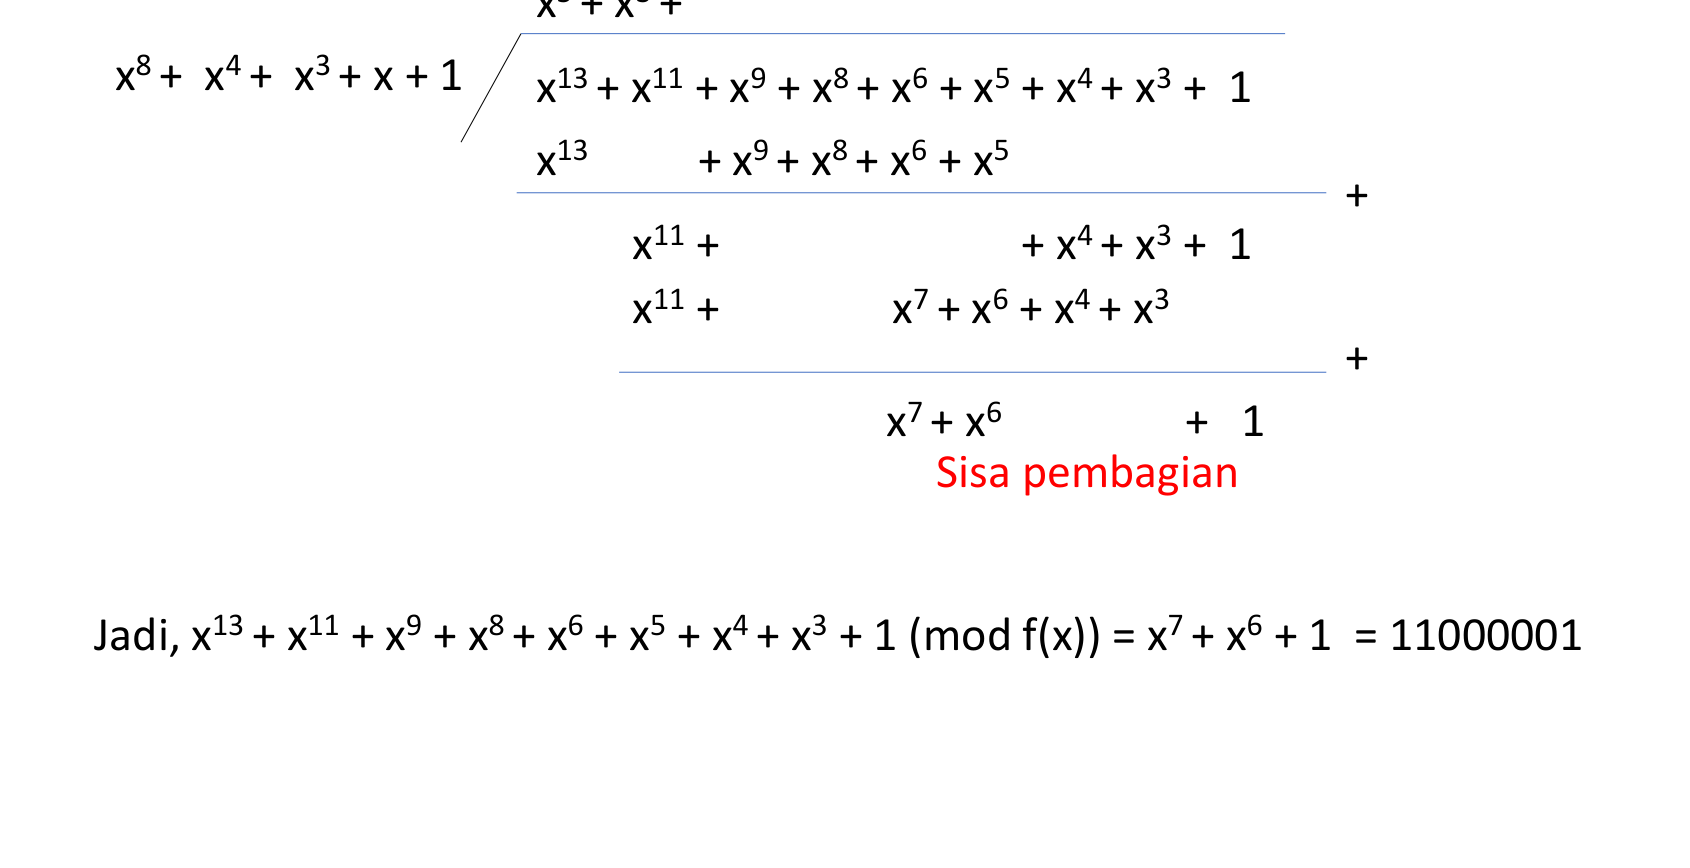
\includegraphics[width=184.80mm,height=238.79mm]{../../images/llm/page_059_img_01.png}%
\end{textblock*}

% bbox perkiraan otomatis: Proses pembagian polinomial dalam aritmatika biner (GF(2)) untuk mencari sisa pembagian (modulo).

\end{document}
